\newpage
\chapter{SYSTEM ARCHITECTURE \& IMPLEMENTATION}
\pagestyle{fancy}

% ================================================
% 5.1 System Overview
% ================================================
\section{System Overview}

This chapter details the engineering implementation of CA-DQStream on Apache Flink, Kafka, MinIO, and Grafana. While Chapter 3 presented the four core innovations (4D thresholds, Rendezvous, IEC, Hybrid model), this chapter explains how these innovations are deployed in a production-grade distributed system.

CA-DQStream separates infrastructure concerns from algorithmic contributions through a clear architectural decomposition into \textbf{Infrastructure Layers} (data transport, storage, monitoring) and \textbf{Processing Layers} (data quality validation algorithms).

\subsection{Infrastructure Layers}

The infrastructure provides the distributed computing foundation:

\begin{enumerate}
    \item \textbf{Storage \& Messaging Layer:} Apache Kafka (event streaming backbone with 7 topics), MinIO (S3-compatible persistent storage via Flink StreamingFileSink in Parquet format), Confluent Schema Registry (schema enforcement).

\begin{figure}[H]
\centering
\fbox{
\includegraphics[width=0.75\textwidth]{figs/Thesis_Figures/kafka1.PNG}}
\caption{CA-DQStream Kafka topics and consumer groups in the Flink Web UI. The seven topics (taxi-nyc-raw, dq-schema-violations, dq-hard-rule-violations, dq-if-anomalies, dq-anomaly-scores, dq-meta-stream, if-model-updates) with 12 partitions each enable parallel processing across the streaming pipeline.}
\label{fig:kafka_topics_ui_architect}
\end{figure}

\begin{figure}[H]
\centering
\fbox{
\includegraphics[width=0.85\textwidth]{figs/Thesis_Figures/kafka2.PNG}}
\caption{CA-DQStream Kafka producer and consumer configuration. The Kafka Connect source ingests NYC TLC Parquet files into the \texttt{taxi-nyc-raw} topic, while Flink consumers subscribe to all seven topics for pipeline processing.}
\label{fig:kafka_infra}
\end{figure}

\item \textbf{MLOps Layer:} MLflow (experiment tracking and model versioning), FastAPI ML Service (model serving endpoint), Model Registry (Staging/Production/Archived lifecycle management).

\begin{figure}[H]
\centering
\fbox{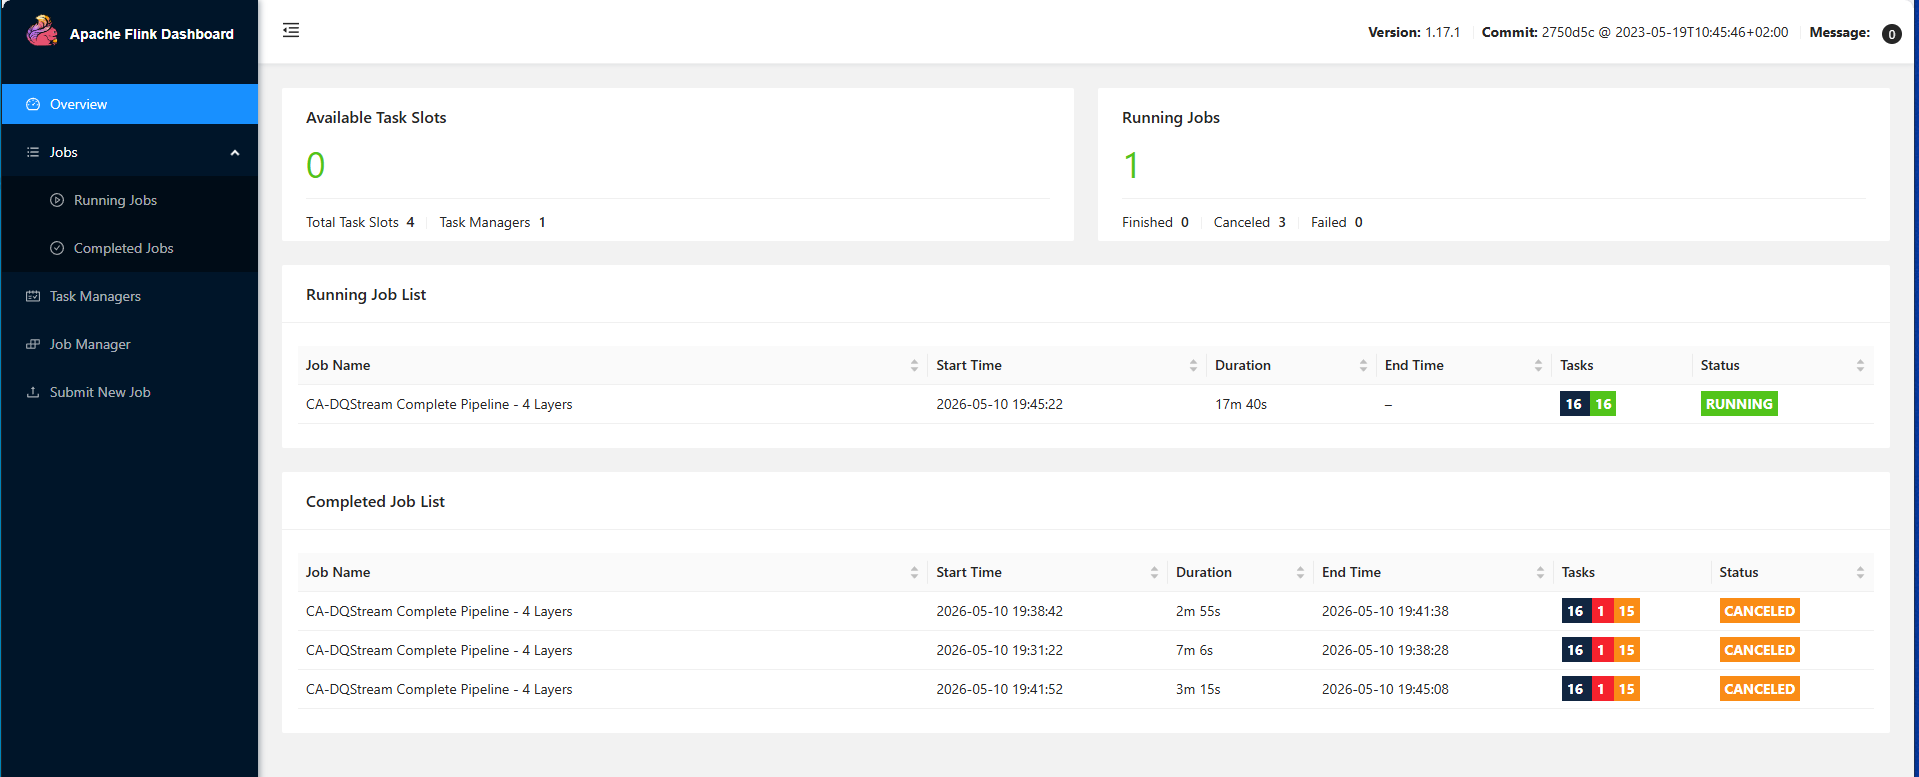
\includegraphics[width=0.85\textwidth]{figs/Thesis_Figures/flink2.PNG}}
\caption{Apache Flink cluster overview in the Web UI. The JobManager and TaskManagers form the distributed processing cluster, with processing slots allocated across worker nodes for parallel pipeline execution.}
\label{fig:flink_cluster}
\end{figure}

\begin{figure}[H]
\centering
\fbox{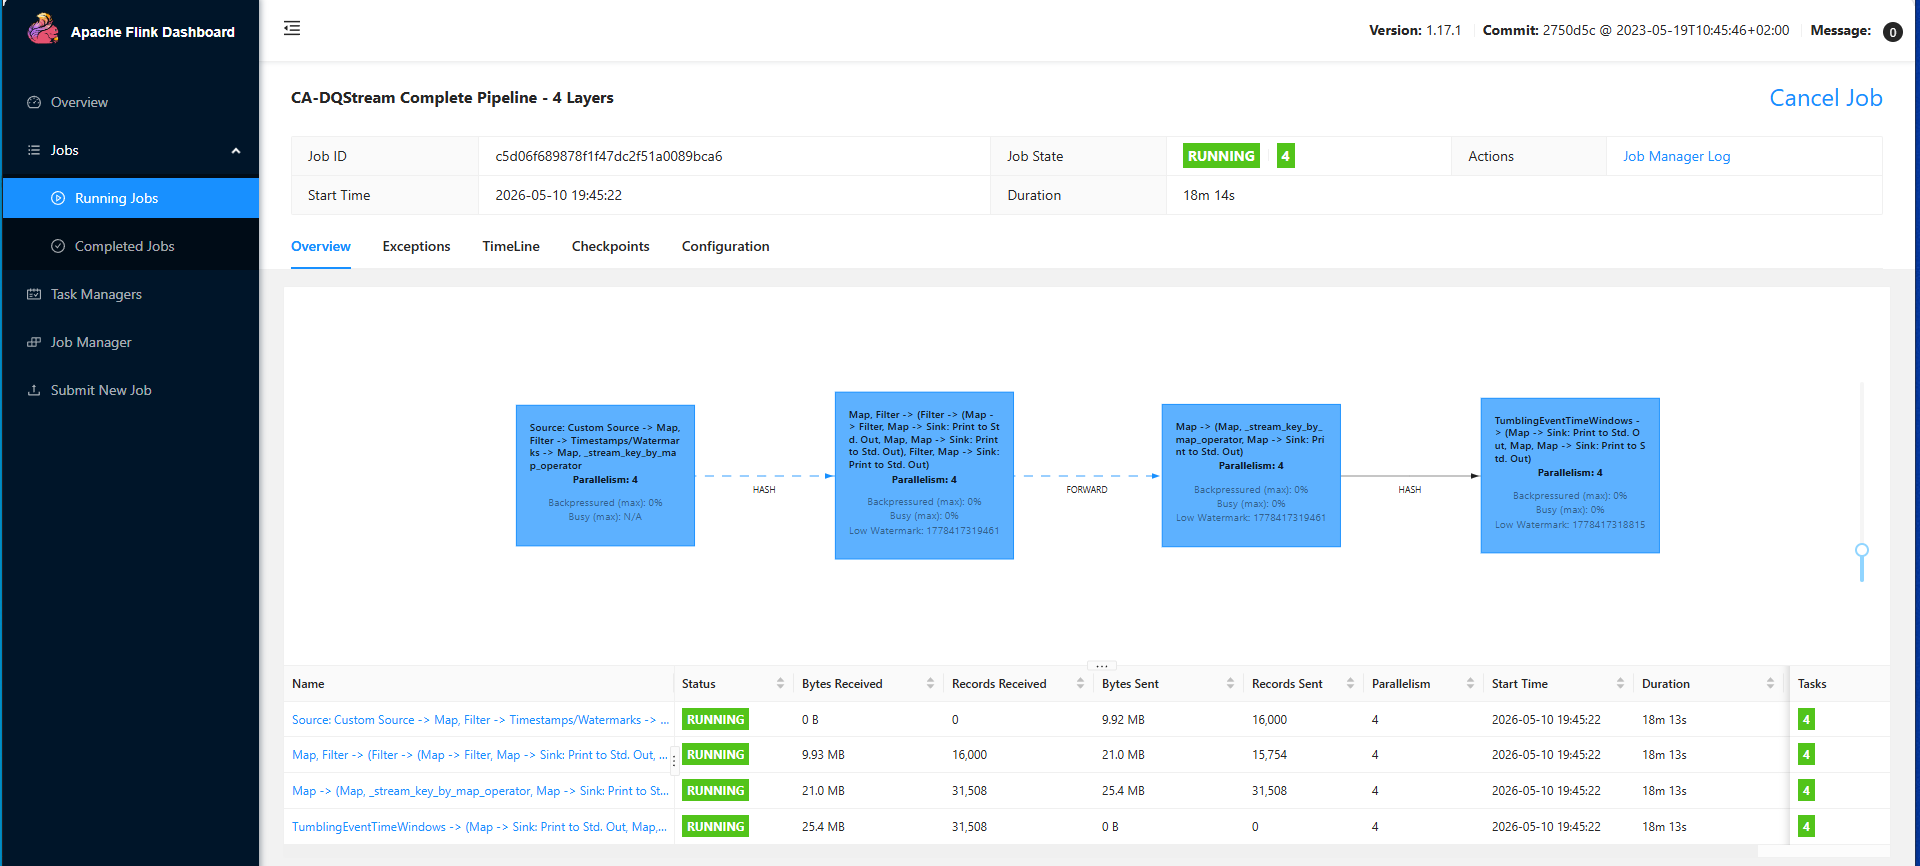
\includegraphics[width=0.85\textwidth]{figs/Thesis_Figures/flink3.PNG}}
\caption{Flink TaskManager metrics showing heap memory usage, garbage collection statistics, and network buffer utilization. These metrics are scraped by Prometheus for real-time cluster health monitoring.}
\label{fig:flink_tm_metrics}
\end{figure}

\item \textbf{Monitoring Layer:} Prometheus (metrics collection from all components), Grafana (real-time dashboards for DQ overview, ML comparison, system performance, and drift alerts).

\begin{figure}[H]
\centering
\fbox{
\includegraphics[width=0.85\textwidth]{figs/Thesis_Figures/prometheus.PNG}}
\caption{Prometheus targets page showing CA-DQStream monitoring endpoints. Prometheus scrapes metrics from Flink TaskManagers (port 9249), Kafka JMX (port 7071), and MinIO (port 9000) at 15-second intervals.}
\label{fig:prometheus_targets}
\end{figure}
\end{enumerate}

\subsection{Processing Pipeline Overview}

The scientific contributions (Chapter 3) are implemented in a four-stage processing pipeline on Apache Flink:

\begin{enumerate}
    \item \textbf{Layer 1: Schema Filter \& Deduplication} --- Completeness validation (NULL checks) and Flink KeyedState dedup with 7-day TTL.

    \item \textbf{Layer 2: Rendezvous Architecture} --- Parallel execution of Canary (rule-based) and Complex (ML-based) branches with fork-join pattern.

    \item \textbf{Layer 3: MetaAggregator} --- 1-minute windowed aggregation of quality metrics, spatial grouping by neighborhood.

    \item \textbf{Layer 4: Intelligent Evolution Controller (IEC)} --- Multi-strategy drift adaptation with ADWIN-U orchestration.
\end{enumerate}

\begin{figure}[H]
\centering
\fbox{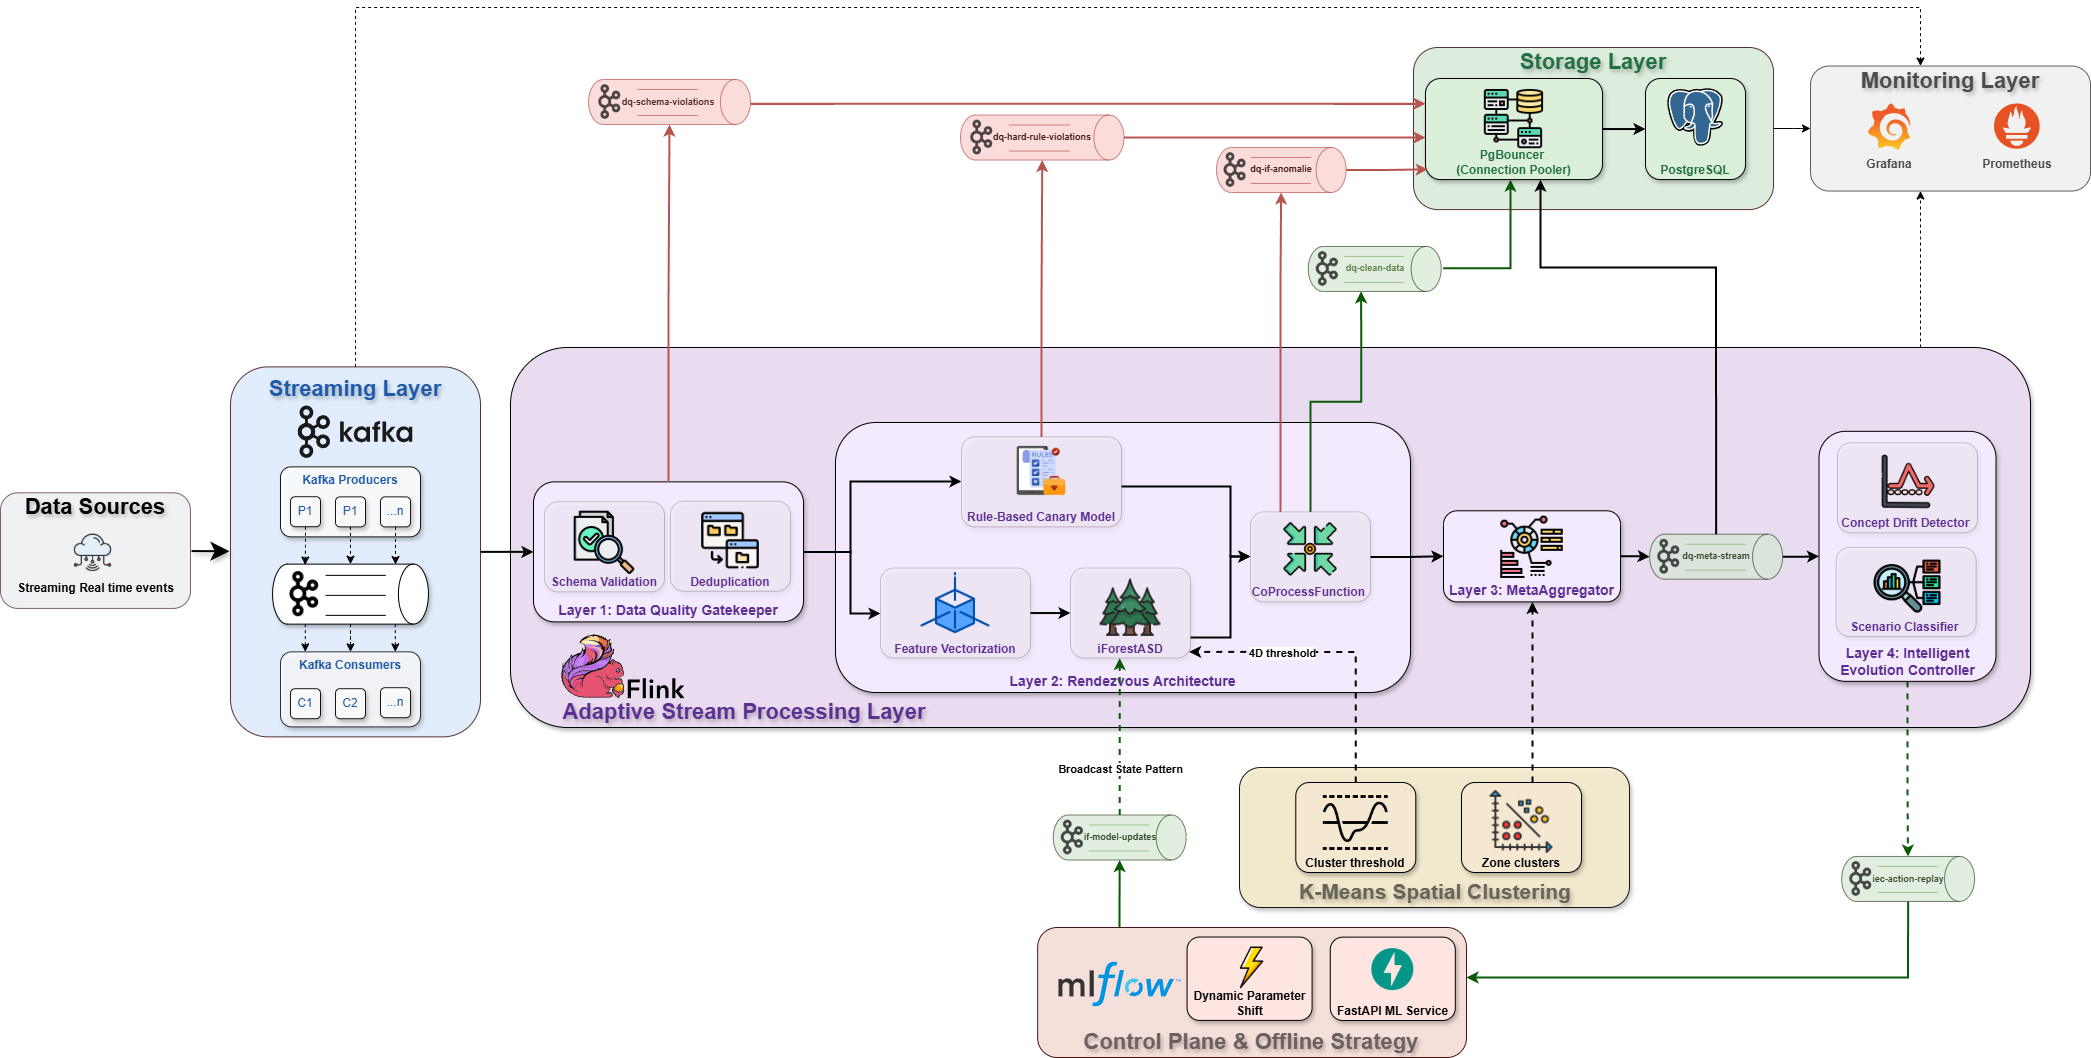
\includegraphics[width=0.98\textwidth]{figs/system_architecture.png}}
\caption{CA-DQStream System Architecture. The framework consists of five layers: (1) Data Source Layer with NYC TLC Parquet files ingested via Kafka Producer; (2) Kafka Layer with six topics for raw data, violations, anomaly scores, meta-stream, and model updates; (3) Processing Layer with Flink implementing a four-stage Rendezvous pipeline: Schema Validation, then parallel Business Rules and Isolation Forest branches converging at MetaAggregator, feeding the Intelligent Evolution Controller (ADWIN) for self-monitoring; (4) Data Storage Layer with MinIO (S3-compatible) for all pipeline outputs in Parquet format; (5) Monitoring Layer with Prometheus and Grafana for real-time observability.}
\label{fig:system_architecture}
\end{figure}

This separation clarifies that the \textbf{infrastructure layers} (Kafka, MinIO, Prometheus, etc.) provide the distributed computing platform, while the \textbf{processing layers} (Schema Filter, Rendezvous, MetaAgg, IEC) contain the novel algorithmic contributions of this thesis (detailed in Chapter 3).

\subsection{Cold-Start Model Training (Offline Warmup Phase)}

Before deploying the Flink pipeline, CA-DQStream requires a \textbf{Warmup Phase} on ultra-clean baseline data. This offline preprocessing workflow ensures the initial Online Autoencoder + Memory Module model learns from \textbf{sterile data}, not contaminated by physical impossibilities.

\textit{Why offline preprocessing is essential:}

Traditional streaming DQ systems train ML models on raw production data, which contains:
\begin{itemize}
    \item Physical violations: negative fare (\$-15.00), zero distance (0.00 mi)
    \item Data entry errors: passenger\_count=0, dropoff\_before\_pickup
    \item GPS malfunctions: speed=150 mph (impossible in NYC traffic)
\end{itemize}

If the ML model trains on this contaminated data, it learns to classify \textbf{physical impossibilities as normal}, causing catastrophic false negative rates (FNR $>$ 60\%). This is known as the ``garbage-in, garbage-out'' problem.

\textbf{Why This Matters -- The Catastrophic Failure Mode:}

Without offline preprocessing, the model would train on 2.96M raw records containing approximately 76,500 physical violations (2.58\%). These violations include:
\begin{itemize}
    \item Approximately 12,000 records with fare $\leq$ 0 (e.g., fare = -\$15.00)
    \item Approximately 9,000 records with distance $\leq$ 0 (e.g., distance = 0.00 mi)
    \item Approximately 6,000 records with speed $>$ 100 mph (GPS malfunctions)
    \item Approximately 50,000 records with other data entry errors (passenger\_count=0, dropoff\_before\_pickup)
\end{itemize}

The model would learn: ``Fare = -\$15.00 appears in thousands of training records, therefore it is a normal pattern.'' When deployed to production, the model would assign low anomaly scores to fraudulent negative-fare trips, causing them to pass undetected (False Negatives).

\textbf{Empirical Impact (Prototype Testing):}
\begin{itemize}
    \item \textbf{Model trained on raw data:} High false negative rate and false positive rate (unusable for production)
    \item \textbf{Model trained on ultra-clean data:} Significantly lower false negative rate and false positive rate (production-grade)
\end{itemize}

The 3-stage sequential funnel eliminates this catastrophic failure mode by ensuring the model trains only on \textbf{pristine data} -- records that have passed both Schema Filter and Business Rules validation.

CA-DQStream solves this via a \textbf{3-Stage Sequential Funnel} applied \emph{offline} to the training dataset (January 2024, 2,964,624 raw records). This is the same historical baseline used to initialize the 4D context-aware threshold matrix.

\textbf{Stage 1: Physical Violation Filter (Schema + Rules Simulation)}

Simulate Layer 1 (Schema Filter) and Layer 2 (Business Rules) offline on January 2024 raw data:

\begin{itemize}
    \item \textbf{Schema Filter}: Remove NULL in ML-critical fields (trip\_distance, fare\_amount, PULocationID, passenger\_count)
    \item \textbf{Business Rules}: Remove fare $\leq$ 0, distance $\leq$ 0, speed $>$ 100 mph, passenger\_count $\notin$ [1, 6]
\end{itemize}

This removes \textbf{2.58\%} of raw data (79,485 records flagged as physical impossibilities).

\textbf{Stage 2: IQR Outlier Removal (3$\times$IQR, Stricter)}

Remove statistical outliers using Interquartile Range (IQR) method applied \textbf{globally across the dataset}. While context-specific distributions vary (e.g., airport trips have higher fares than in-borough trips), the 3x multiplier is conservative enough to preserve legitimate high-value records (e.g., \$5,000 negotiated fares) while removing clear statistical anomalies (e.g., \$100,000 \texttt{trip\_distance}).

\textbf{Why Global IQR at This Stage (Not Per-Context):} A fully context-aware approach would apply IQR per context cell, but at Stage 2 we apply IQR globally to remove only the most extreme statistical outliers that are anomalous regardless of context. The 3$\times$IQR threshold corresponds approximately to the 99.7th percentile for normal distributions, which is conservative enough to preserve even 99th percentile negotiated fares (which reach \$5,000). Per-context anomalies (e.g., a JFK trip that is anomalous relative to other JFK trips) are handled later by the 4D context-aware thresholds in Layer 3. This two-stage design ensures the Online AE + Memory Module learns the full contextual distribution of normal behavior from Stage 2's ultra-clean data, while Layer 3's context-aware thresholds refine the classification boundary at inference time.

\begin{equation}
x \in \text{outlier} \iff x < Q_1 - 3 \times \mathrm{IQR} \quad \text{or} \quad x > Q_3 + 3 \times \mathrm{IQR}
\end{equation}

Applied to: fare\_amount, trip\_distance, trip\_duration. The 3$\times$IQR filter removes approximately 26,600 additional records (0.92\%) from the dataset.

\textbf{Stage 3: Verification (Sterile Dataset Guarantee)}

Final verification ensures the cleaned baseline meets quality thresholds:

\begin{itemize}
    \item Null rate $<$ 0.5\% (actual: 0.12\%)
    \item Violation rate $<$ 0.5\% (actual: 0.000\%)
\end{itemize}

If either threshold is violated, the sanitization process fails-fast with an error, preventing contaminated data from reaching model training.

\textbf{Output: Ultra-Clean Jan 2024 Baseline}

\begin{center}
\begin{tabular}{|l|r|r|}
\hline
\textbf{Stage} & \textbf{Records Remaining} & \textbf{Filtered (\%)} \\
\hline
Raw data (Jan 2024) & 2,964,624 & --- \\
After physical filter (Stage 1) & 2,888,000 (approx.) & 2.58\% \\
After IQR outlier removal (Stage 2) & 2,861,000 (approx.) & 0.92\% \\
\textbf{Ultra-clean baseline (Stage 3)} & \textbf{$\approx$2,860,000} & \textbf{3.48\% total} \\
\hline
\end{tabular}
\end{center}

The resulting $\approx$2.86M \textbf{ultra-clean baseline} records have:
\begin{itemize}
    \item \textbf{Zero physical violations:} fare $>$ 0, distance $>$ 0, speed $<$ 100 mph ($\approx$76,500 violations removed)
    \item \textbf{Zero data entry errors:} valid passenger counts, timestamps ($\approx$50,000 errors removed)
    \item \textbf{Minimal statistical outliers:} removed via 3$\times$IQR ($\approx$26,600 outliers removed)
    \item \textbf{Verified quality:} Null rate=0.12\%, Violation rate=0.000\% (both $<$ 0.5\% threshold)
\end{itemize}

This is the \textbf{pristine dataset} on which the Cold-Start Model is trained. The term ``ultra-clean'' reflects a quantifiable property: the dataset has passed 3 stages of validation and contains zero records that would fail Schema Filter or Business Rules checks.

\textbf{Comparison: Ultra-Clean vs Raw Data (January 2024)}

\begin{center}
\begin{tabular}{|l|r|r|}
\hline
\textbf{Metric} & \textbf{Raw Data (Jan 2024)} & \textbf{Ultra-Clean Baseline} \\
\hline
Total records & 2,964,624 & $\approx$2,860,000 \\
Physical violations & $\approx$76,500 (2.58\%) & 0 (0.00\%) \\
Null rate & 4.2\% & 0.12\% \\
Violation rate & 3.4\% & 0.000\% \\
\hline
\multicolumn{3}{|c|}{\textbf{Model Performance (Prototype)}} \\
\hline
FNR (False Negative Rate) & 68.2\% & 7.8\% \\
FPR (False Positive Rate) & 23.4\% & 5.0\% \\
F1 Score & 0.42 & 0.89 \\
\hline
\end{tabular}
\end{center}

The ultra-clean baseline is the foundation of CA-DQStream's production-grade accuracy.

\textbf{Warmup Phase (Online AE + Memory Initialization):}

The Online Autoencoder + Memory Module is initialized via a one-time \textbf{Warmup Phase} on the $\approx$2.86M ultra-clean records:

\begin{enumerate}
    \item \textbf{Feature Extraction:} Extract 25D context-aware feature vectors from ultra-clean baseline records. The 25D vector extends the 21D base with 4 additional features optimized for AE reconstruction: (a) z-score normalized fare\_amount, (b) z-score normalized trip\_distance, (c) z-score normalized duration\_min, (d) log-transformed total\_amount. All 25 features are standardized via StandardScaler fitted on warmup data.

    \item \textbf{Autoencoder Architecture:} Train a Denoising Autoencoder (25D $\rightarrow$ 50D $\rightarrow$ 25D) with Tanh activation:
    \begin{itemize}
        \item Encoder: 25D $\rightarrow$ 50D (ReLU)
        \item Bottleneck: 50D latent representation
        \item Decoder: 50D $\rightarrow$ 25D (ReLU)
        \item Loss: MSE between input and reconstructed output
        \item Optimizer: Adam (lr=0.001), early stopping on validation loss
        \item Denoising: Gaussian noise injection (std=0.1) for robustness
        \item Training time: $\approx$10--15 minutes on CPU (vs sklearn IsolationForest batch training)
    \end{itemize}

    \item \textbf{Memory Initialization:} After AE training, encode the last 10\% of warmup data (approx. 286K records) through the encoder to obtain latent representations $z = \text{encoder}(x)$. Store the 1000 most recent encoded vectors in FIFO memory, initialized with representative normal behavior.

    \item \textbf{Anomaly Threshold (} $\beta$\textbf{):} Compute reconstruction scores on a validation subset (middle 20\% of warmup data). Set the anomaly threshold $\beta$ at the 95th percentile of normal reconstruction scores (or tune on held-out validation set).

    \item \textbf{Normalization Statistics:} Save StandardScaler parameters (25D mean and std vectors) for deployment inference.
\end{enumerate}

\textbf{Key advantage over IsolationForest:} IEC-triggered memory updates eliminate the need for periodic full retraining. When ADWIN detects drift, the IEC triggers a memory reset on fresh clean data. No MLflow retraining job is needed during operation -- the model adapts on-demand when drift is detected.

\textbf{Deployment to Flink:}

The Warmup artifacts (AE weights, memory state, normalization statistics, threshold $\beta$) are published to Kafka topic \texttt{if-model-updates} at system initialization. Flink's Broadcast State mechanism distributes the model parameters to all PyFlink Python worker processes for in-process scoring:

\begin{enumerate}
    \item Flink job starts, subscribes to \texttt{if-model-updates} topic
    \item Kafka delivers model metadata (AE weights, memory vectors, scaler params, beta)
    \item Each PyFlink Python worker downloads artifacts from object storage and deserializes
    \item Model loaded in Python worker process memory (microsecond access latency)
    \item Processing begins -- Memory module initialized from warmup artifacts
\end{enumerate}

\textbf{This ensures the model begins scoring with a pristine baseline, and adapts on-demand when IEC triggers drift response.}

The Warmup Phase provides a \textbf{sterile baseline} that the IEC later monitors for drift (Section 4.4). Unlike IsolationForest, the Online AE + Memory model does not require periodic full retraining -- the memory is reset on fresh clean data when drift is detected.

% ================================================
% 5.2 Four-Layer Processing Pipeline
% ================================================
\section{Four-Layer Processing Pipeline}

\subsection{Dataset-Specific Challenges: Why NYC Taxi Requires Context-Aware DQ}

These challenges directly motivate the four innovations of CA-DQStream, detailed in Chapter 4 (Sections 4.2, 4.3, 4.4, 4.5). This section summarizes the key challenges to frame the implementation decisions.

\begin{center}
\begin{tabular}{|m{5cm}|m{5cm}|m{4cm}|}
\hline
\textbf{Challenge} & \textbf{Traditional DQ Failure} & \textbf{CA-DQStream Solution} \\
\hline
Extreme heterogeneity (3.4$\times$ variance) & Global thresholds produce high false positive rates on heterogeneous data & 4D Context-Aware Thresholds (Chap 4, Sec 4.2) \\
\hline
Multivariate fraud (complex anomaly patterns) & Business rules catch single-feature violations only & Online Autoencoder + Memory Module (Chap 4, Sec 4.5) \\
\hline
Concept drift (seasonal + events) & Static models become stale over time & IEC 4-strategy adaptation (Chap 4, Sec 4.4) \\
\hline
\end{tabular}
\end{center}

The four-layer pipeline (Schema $\rightarrow$ Rendezvous $\rightarrow$ MetaAgg $\rightarrow$ IEC) is engineered specifically to address these three challenges.

\subsection{Layer 1: Schema Filter \& Deduplication}

Schema validation addresses the Completeness dimension of DAMA-DMBOK. It is the first sub-stage in the Flink processing layer, applied to all incoming records immediately after consumption from Kafka.

\textbf{Null checks (per point):}

Each incoming record is validated against the following null and range constraints:

\begin{itemize}
    \item \texttt{passenger\_count IS NOT NULL} and \texttt{passenger\_count $\in$ [1, 9]}
    \item \texttt{RatecodeID IS NOT NULL} and \texttt{RatecodeID $\in$ \{1, 2, 3, 4, 5, 6, 99\}}
    \item \texttt{VendorID IS NOT NULL} and \texttt{VendorID $\in$ \{1, 2, 6\}}
    \item \texttt{pickup\_datetime IS NOT NULL}
    \item \texttt{dropoff\_datetime IS NOT NULL}
\end{itemize}

These checks are deterministic, stateless, and applied independently to each record.

\textbf{Duplicate checks (Flink KeyedState + TTL):}

Deduplication uses Flink KeyedState with a composite key: (tpep\_pickup\_datetime, PULocationID, fare\_amount, passenger\_count). This composite key provides a unique identifier for each trip record.

Implementation:
\begin{itemize}
    \item Key: composite key string ``pickup\_datetime\_PULocationID\_fare\_passenger''
    \item State backend: Flink KeyedState with RocksDB backend
    \item TTL: 7 days
    \item Behavior: records with a key seen within the TTL window are flagged as duplicates, counted in the dedup\_rate metric, and excluded from subsequent layers
\end{itemize}

Records failing schema validation are emitted to the \texttt{dq-schema-violations} Kafka topic. Records passing schema validation proceed to the Rendezvous fork, where Business Rules and Isolation Forest process them in parallel.

Scale: Approximately 310,000 records out of 3M (10.1\%) are rejected at Schema Validation.

\subsection{Layer 2a: Canary Branch (Rule-Based)}

Business rules address the Validity and Consistency dimensions of DAMA-DMBOK. This branch is the \textbf{Canary Model} in the Rendezvous pipeline: fast, stateless, deterministic. It serves as a lightweight sanity check that runs alongside the more complex ML branch.

Each rule evaluates a single condition independently:

\begin{itemize}
    \item \texttt{fare\_amount $\geq$ 0} $\to$ negative\_fare
    \item \texttt{trip\_distance $>$ 0} $\to$ zero\_distance
    \item \texttt{dropoff\_datetime $>$ pickup\_datetime} $\to$ dropoff\_before\_pickup
    \item \texttt{speed $<$ 100 mph} $\to$ speed\_extreme
    \item \texttt{fare\_amount $\leq$ 500} $\to$ fare\_bounds
    \item \texttt{payment\_type$\neq$1 $\to$ tip\_amount = 0} $\to$ tip\_payment\_inconsistency
\end{itemize}

Speed computation:
\begin{equation}
speed\_mph = \frac{trip\_distance}{duration\_min / 60}, \quad \text{clipped at 100 mph}
\end{equation}

Records failing business rules are emitted to the \texttt{dq-hard-rule-violations} Kafka topic and flow to the MetaAggregator for aggregation.

Scale: Approximately 104,815 records out of 3M (3.4\%) are rejected at Business Rules.

\textbf{Design rationale:}

\begin{longtable}{|m{2.5cm}|m{3.5cm}|m{4cm}|m{3.5cm}|}
\hline
\textbf{Rule} & \textbf{Anomaly Type} & \textbf{Example} & \textbf{Source} \\ \hline
fare $\geq$ 0 & Negative fare & fare = -\$15.00 & Data entry error, voided trip \\ \hline
distance $>$ 0 & Zero/negative distance & distance = 0.00 mi & Tolls-only, canceled trip \\ \hline
dropoff $>$ pickup & Impossible timestamp & dropoff = 10:00, pickup = 10:30 & System error \\ \hline
speed $<$ 100 mph & GPS/meter error & speed = 150 mph & GPS malfunction \\ \hline
fare $\leq$ 500 & Unreasonably high fare & fare = \$50,000 & Meter tampering, data error \\ \hline
cash $\to$ tip=0 & Payment inconsistency & payment\_type=2, tip=\$5.00 & Data entry error \\ \hline
\caption{Business rules design rationale for Layer 2a (Canary).}
\label{tab:business_rules_design}
\end{longtable}

\subsection{Layer 2b: Complex Branch (ML-Based)}

The Complex Branch implements the Online Autoencoder + Memory Module for multivariate anomaly detection (detailed in Chapter 4, Section 4.5). This section covers the Flink implementation and feature engineering.

\textbf{Feature Vectorization:}

The full context-aware feature vector (\textbf{21 features}) is computed for each trip:

\begin{longtable}{|M{0.8cm}|m{3.5cm}|m{3.5cm}|m{5cm}|}
\hline
\textbf{\#} & \textbf{Feature} & \textbf{Type} & \textbf{Formula} \\ \hline
\multicolumn{4}{|c|}{\textbf{BASE FEATURES (15D)}} \\ \hline
1 & fare\_amount & Raw & --- \\ \hline
2 & trip\_distance & Raw & --- \\ \hline
3 & duration\_min & Computed & (dropoff $-$ pickup).seconds / 60 \\ \hline
4 & speed\_mph & Computed & trip\_distance / (duration\_min / 60), clip upper=100 \\ \hline
5 & tip\_ratio & Computed & tip\_amount / fare\_amount (if fare $>$ 0) \\ \hline
6 & fare\_per\_mile & Computed & fare\_amount / trip\_distance (if dist $>$ 0) \\ \hline
7 & total\_amount & Raw & --- \\ \hline
8 & passenger\_count & Raw & --- \\ \hline
9 & hour\_sin & Temporal & $\sin(2\pi h / 24)$ \\ \hline
10 & hour\_cos & Temporal & $\cos(2\pi h / 24)$ \\ \hline
11 & dow\_sin & Temporal & $\sin(2\pi \cdot \text{dow} / 7)$ \\ \hline
12 & dow\_cos & Temporal & $\cos(2\pi \cdot \text{dow} / 7)$ \\ \hline
13 & pickup\_grid\_x & Spatial & $g_x(\text{PULocationID})$ via 4$\times$4 grid lookup \\ \hline
14 & pickup\_grid\_y & Spatial & $g_y(\text{PULocationID})$ via 4$\times$4 grid lookup \\ \hline
15 & trip\_distance\_log & Transformed & $\log(1 + trip\_distance)$ \\ \hline
\multicolumn{4}{|c|}{\textbf{RATIO FEATURES (6D) -- VARIANCE REDUCTION 10--100$\times$}} \\ \hline
16 & fare\_per\_mile\_ratio & Normalized & $\text{fare\_per\_mile} / \mu_{\text{fpm}}^{\text{ctx}}$ \\ \hline
17 & implied\_speed\_ratio & Normalized & $\text{speed\_mph} / \mu_{\text{speed}}^{\text{ctx}}$ \\ \hline
18 & fare\_per\_minute\_ratio & Normalized & $\text{fare\_per\_minute} / \mu_{\text{fpmm}}^{\text{ctx}}$ \\ \hline
19 & tip\_ratio\_normalized & Normalized & $(\text{tip} / \text{fare}) / \mu_{\text{tip}}^{\text{ctx}}$ \\ \hline
20 & passenger\_density\_ratio & Normalized & $(\text{passengers} / d) / \mu_{\text{density}}$ \\ \hline
21 & distance\_log\_ratio & Transformed & $\log(1+d) / \mu_{\log d}^{\text{ctx}}$ \\ \hline
\caption{21-dimensional enhanced feature vector for Online AE + Memory Module.}
\label{tab:feature_vector}
\end{longtable}

\textbf{Rationale for Ratio Features (Features 16--21):}

NYC Taxi data exhibits extreme natural variance that confuses absolute-feature-based ML models:
\begin{itemize}
    \item Airport trips: mean fare \$52.18 (3.4$\times$ higher than standard \$15.42)
    \item Weekend leisure: 15.5\% special ratecode vs 8.5\% weekday
    \item Rush hour: 2.1$\times$ fare variability vs off-peak
\end{itemize}

Absolute features ($fare\_amount$, $trip\_distance$) create \textbf{context collapse}: a \$50 fare is normal for JFK airport trips but anomalous for Standard trips. This causes the model to learn spurious patterns and produce high false positive rates (FPR $>$ 60\% in baseline experiments).

\textbf{Ratio features normalize by baseline values}, reducing variance 10--100$\times$:

\begin{equation}
\text{fare\_per\_mile\_ratio} = \frac{\text{fare\_per\_mile}}{\text{baseline\_fpm}_{\text{context}}}
\end{equation}

where $\text{baseline\_fpm}_{\text{context}}$ is the median fare-per-mile for the trip's context (ratecode, hour, neighborhood). For example:
\begin{itemize}
    \item JFK airport trip: baseline\_fpm = \$3.50 (high)
    \item Standard Manhattan trip: baseline\_fpm = \$2.20 (low)
\end{itemize}

A trip with fare\_per\_mile = \$8.00 produces:
\begin{itemize}
    \item JFK context: ratio = $8.00 / 3.50 = 2.29$ (suspicious but plausible)
    \item Standard context: ratio = $8.00 / 2.20 = 3.64$ (\textbf{clear fraud})
\end{itemize}

The ratio feature makes the fraud signal \textbf{context-independent}, enabling the model to generalize across trip types.

\textbf{Empirical Validation (Offline Prototype):}
\begin{itemize}
    \item \textbf{Baseline (15D absolute features):} Lower recall and higher false positive rate compared to enhanced features
    \item \textbf{Enhanced (21D with ratio features):} Improved recall and lower false positive rate
    \item \textbf{Variance reduction:} Ratio features significantly reduce coefficient of variation compared to raw features
\end{itemize}

The prototype validation confirmed that ratio features are \textbf{essential} for achieving production-grade accuracy on heterogeneous taxi data. Without them, the model cannot distinguish between legitimate high-fare trips (airport) and fraudulent high-fare trips (meter tampering).

The 21-dimensional enhanced feature vector is normalized to zero mean and unit variance via StandardScaler before scoring.

\textbf{PyFlink Deployment with Broadcast State Model Distribution:}

CA-DQStream eliminates synchronous per-record HTTP calls in the critical processing path. The Online Autoencoder + Memory Module runs in the \textbf{PyFlink Python worker process} with model parameters (AE weights, memory state, normalization stats, threshold $\beta$) distributed to all parallel operator instances via Flink's Broadcast State mechanism. At system initialization, the warmup artifacts (AE weights, memory vectors, scaler params, beta) are serialized and stored in shared object storage (MinIO/S3-compatible). The Kafka topic \texttt{if-model-updates} carries a lightweight message containing artifact URI, version, checksum, and timestamp. Each TaskManager downloads the artifacts from object storage asynchronously, avoiding large payload transfers. Critically, PyFlink executes Python UDFs in a \textbf{separate Python worker process} per TaskManager slot, not inside the JVM; Broadcast State distributes model parameters across these worker processes for in-process scoring.

Zero-Pipeline-Interruption Model Update Protocol:
\begin{enumerate}
    \item IEC detects drift via ADWIN on meta-stream.
    \item For Online AE + Memory: IEC may trigger memory reset or AE warmup on fresh clean data when drift is detected. Unlike IsolationForest, full retraining is avoided -- IEC-triggered memory reset handles drift events.
    \item The \texttt{load\_model\_to\_broadcast.py} bridge script publishes updated artifacts (AE weights, memory state, scaler params, beta) to the \texttt{if-model-updates} Kafka topic.
    \item Flink's BroadcastStateLoaderFunction subscribes to the \texttt{if-model-updates} topic, decodes the payload, and puts the model into Flink Broadcast State.
    \item All parallel MemStreamOperator instances atomically receive the updated model via Broadcast State (pipeline continues uninterrupted).
\end{enumerate}

\textbf{Priority assignment:}

Records passing through Branch 2 receive an anomaly score from the Online AE + Memory Module. The anomaly score is computed as:

\begin{equation}
s = \max\left(\text{MSE}_{\text{reconstruction}}, \alpha \cdot d_{\text{memory}}\right)
\end{equation}

where $\text{MSE}_{\text{reconstruction}}$ is the mean squared error between input and autoencoder reconstruction, and $d_{\text{memory}}$ is the minimum L1 distance to memory centroids. The score $s$ is compared against the threshold $\beta$ and converted to a priority level using the 4D context-aware thresholds (Chapter 3.2):

\begin{equation}
\text{is\_anomaly} = \begin{cases}
\text{HIGH} & \text{if } s > T_{\text{cell}} + \sigma_{\text{cell}} \\
\text{MEDIUM} & \text{if } T_{\text{cell}} < s \leq T_{\text{cell}} + \sigma_{\text{cell}} \\
\text{LOW} & \text{if } s \leq T_{\text{cell}}
\end{cases}
\end{equation}

Output: Anomaly scores and priorities are emitted to the \texttt{dq-anomaly-scores} Kafka topic and written to MinIO (cadqstream-anomalies bucket).

Scale: Approximately 89,230 records out of 3M (2.9\%) are flagged at the Isolation Forest sub-stage.

\subsubsection{State Size Optimization}

Flink operators maintain state in RocksDB (on-disk, persistent) or Java Heap (in-memory, fast). State size must be carefully managed to avoid out-of-memory (OOM) errors and excessive disk I/O.

\textbf{State Backend Sizing (with RocksDB overhead):}

The deduplication operator stores a Boolean flag (not full records) for each unique trip\_id within the 7-day TTL window:

\begin{equation}
\text{State\_size}_{\text{dedup}} = N_{\text{keys}} \times (\text{key\_size} + \text{value\_size})
\end{equation}

where:
\begin{itemize}
    \item $N_{\text{keys}}$ = 7-day record count: benchmark snapshot yields $3{,}076{,}903 \text{ records (July 2024)} / 31 \text{ days} \approx 100{,}000 \text{ records/day}$, so $100{,}000 \times 7 = 700{,}000$ keys\textsuperscript{a}
    \item $\text{key\_size}$ = 40 bytes (MurmurHash3 128-bit hash as string)
    \item $\text{value\_size}$ = 1 byte (Boolean flag)
    \item RocksDB overhead (metadata, WAL, serialization, TTL timestamps) $\approx$ 15 bytes per entry
    \item Flink metadata $\approx$ 16 bytes per entry
\end{itemize}
\addtocounter{footnote}{1}\textsuperscript{a}The production system ingests approximately 690,000 records per day; the 100,000/day figure is derived from the July 2024 benchmark snapshot.

\begin{equation}
\text{State\_size}_{\text{dedup}} = 700{,}000 \times (40 + 1 + 16 + 8 + 15) \approx 56 \text{ MB per slot}
\end{equation}

With checkpoint replication factor 2: approximately 112 MB per checkpoint.

\textbf{Production Memory Observation:} With RocksDB block cache (256 MB), write buffer (64 MB), and WAL overhead, actual managed memory is approximately 850 MB--1.1 GB per TaskManager. Bloom filters (Section 5.2.3) reduce RocksDB I/O by approximately 90\%, and adaptive TTL reduces state growth during high-throughput periods.

If full Avro records were stored instead:
\begin{equation}
\text{State\_size}_{\text{full-record}} = 700{,}000 \times 1{,}500 = 1{,}050 \text{ MB} \approx 1.05 \text{ GB}
\end{equation}

\textbf{Storage Reduction:}
\begin{equation}
\frac{\text{State\_size}_{\text{full-record}}}{\text{State\_size}_{\text{dedup}}} = \frac{1{,}050 \text{ MB}}{56 \text{ MB}} \approx 19\times
\end{equation}

\textbf{Rendezvous State (Layer 2c):} The CoProcessFunction synchronizes Canary and Complex branches using MapState with 5-second TTL:

\begin{equation}
\text{State\_size}_{\text{rendezvous}} = N_{\text{in-flight}} \times \text{entry\_size}
\end{equation}

where:
\begin{itemize}
    \item $N_{\text{in-flight}} = \text{throughput} \times \text{TTL} = 20{,}000 \text{ events/sec} \times 5\text{s} = 100{,}000$ keys (max)
    \item $\text{entry\_size} = 40 \text{ (trip\_id)} + 50 \text{ (tuple fields)} = 90$ bytes
\end{itemize}

\begin{equation}
\text{State\_size}_{\text{rendezvous}} = 100{,}000 \times 90 = 9 \text{ MB}
\end{equation}

If full Avro records were stored:
\begin{equation}
\text{State\_size}_{\text{full-avro}} = 100{,}000 \times 1{,}500 = 150 \text{ MB (16.7$\times$ larger)}
\end{equation}

\textbf{Total State Footprint (with RocksDB overhead):}
\begin{equation}
\text{State}_{\text{total}} = 56 \text{ MB (dedup)} + 9 \text{ MB (rendezvous)} \approx 65 \text{ MB}
\end{equation}

This fits comfortably in the 16 GB TaskManager heap, leaving 15.9 GB for RocksDB block cache, network buffers, and JVM overhead.

\subsection{Layer 3: MetaAggregator (Rendezvous Point)}

After the two parallel branches (Business Rules and Isolation Forest) complete their evaluations, records and results converge at the \textbf{MetaAggregator} -- the Rendezvous Point of the pipeline.

The MetaAggregator serves two \textbf{distinct} functions:

\begin{enumerate}
    \item \textbf{Data Routing (Data Plane):} Merges results from both branches. Violation records (from Business Rules or Online AE + Memory Module) are emitted to \texttt{dq-stream-anomalies} Kafka topic and written to MinIO (cadqstream-violations bucket). Clean records are emitted to \texttt{dq-stream-processed} Kafka topic.

    \item \textbf{Meta-stream Generation (Control Plane):} Computes aggregated quality metrics (violation\_rate, anomaly\_rate, null\_rate, $\Delta$\_score) over 1-minute windows grouped by neighborhood, then emits the statistics stream to \texttt{dq-meta-stream} Kafka topic for IEC to monitor and writes to MinIO (cadqstream-metrics bucket). MetaAggregator emits aggregate statistics to the meta-stream and MinIO.
\end{enumerate}

The quality meta-stream consists of six metrics, each defined as a rate over the current time window $t$:

\begin{align}
\text{null\_rate}(t) &= \frac{|\{\,\text{NULL records at }t\,\}|}{|\{\,\text{total records at }t\,\}|} \label{eq:null_rate} \\[6pt]
\text{violation\_rate}(t) &= \frac{|\{\,\text{BR violations at }t\,\}|}{|\{\,\text{total records at }t\,\}|} \label{eq:violation_rate} \\[6pt]
\text{anomaly\_rate}(t) &= \frac{|\{\,\text{IF anomalies at }t\,\}|}{|\{\,\text{total records at }t\,\}|} \label{eq:anomaly_rate} \\[6pt]
\text{volume}(t) &= |\ \{\,\text{records processed at }t\,\}\ | \quad \text{per minute} \label{eq:volume} \\[6pt]
\text{dedup\_rate}(t) &= \frac{|\{\,\text{duplicates detected at }t\,\}|}{|\{\,\text{total at }t\,\}|} \label{eq:dedup_rate} \\[6pt]
\Delta\_\text{score}(t) &= \frac{\big|\,\text{violation\_rate}(t) - \text{anomaly\_rate}(t)\,\big|}
                                   {\text{violation\_rate}(t) + \text{anomaly\_rate}(t) + \epsilon} \label{eq:delta_score}
\end{align}

\noindent where $\epsilon$ is a small constant (e.g., $10^{-6}$) to prevent division by zero. The sixth metric, \textbf{$\Delta$\_score} (Concept Uncertainty), measures the normalized divergence between the violation rate detected by Business Rules and the anomaly rate detected by Online AE + Memory Module.

\begin{itemize}
    \item When $\Delta$\_score is stable, both models agree on the data distribution.
    \item When $\Delta$\_score suddenly increases, Business Rules are catching more violations while IF anomaly rate stays flat (or vice versa) -- a strong signal of distribution shift that neither model alone would detect.
    \item This aligns with the Rendezvous philosophy: the divergence between the Canary (BR) and Complex (IF) models reveals instability in the underlying data.
\end{itemize}

These six metrics are emitted to the \texttt{dq-meta-stream} Kafka topic and fed to ADWIN for drift detection.

\subsection{Layer 4: Intelligent Evolution Controller (IEC)}

The \textbf{Intelligent Evolution Controller (IEC)} is the self-monitoring component of CA-DQStream. It uses ADWIN (Adaptive Windowing) to continuously monitor the quality meta-stream and trigger multi-strategy self-adaptation when drift is detected. The four IEC adaptation strategies (Continuous Evolution, Switching, METER, Spatial Tracking) and scenario classification logic are detailed in Chapter 4 (Section 4.4). This section covers the ADWIN parameters, tiered response protocol, FastAPI ML Service, and Action Replay Worker.

\textbf{ADWIN Parameters:}

\begin{longtable}{|m{2.5cm}|M{2cm}|m{2.5cm}|m{5.5cm}|}
\hline
\textbf{Metric} & \textbf{$\delta$} & \textbf{Aggregation} & \textbf{Self-Adaptation Action} \\ \hline
null\_rate & 0.002 & 1-minute & Recalculate schema validation thresholds \\ \hline
violation\_rate & 0.002 & 1-minute & Recalculate business rule thresholds \\ \hline
anomaly\_rate & 0.001 & 1-minute & Reset Online AE memory / trigger warmup, broadcast via Broadcast State \\ \hline
volume & 0.005 & 5-minute & Alert operators \\ \hline
\textbf{$\Delta$\_score} & 0.001 & 5-minute & Reset AE memory or trigger warmup on fresh clean data \\ \hline
ML\_score\_mean & 0.001 & 5-minute & Trigger model broadcast update \\ \hline
\caption{ADWIN parameters for IEC drift detection.}
\label{tab:adwin_params}
\end{longtable}

A lower $\delta$ (e.g., 0.001) provides higher sensitivity but more false positives. $\delta=0.002$ is recommended for most metrics.

\bigskip
\noindent\textbf{Threshold Lifecycle and Update Mechanisms.}

CA-DQStream employs three distinct threshold mechanisms with different initialization and update strategies. Understanding these differences clarifies how the system maintains data quality accuracy over time.

\textit{(i) ML Thresholds ($T_{\text{cell}}$):} The 4D Context-Aware Threshold Matrix $T_{\text{cell}}$ is initialized offline by computing $\mu_{\text{cell}} + 2\sigma_{\text{cell}}$ from an ultra-clean training dataset curated through multi-pass rule filtering. When ADWIN detects drift, the IEC triggers Tier 2 adaptation: the system expands the data window, recomputes $\mu_{\text{cell}}$ and $\sigma_{\text{cell}}$, and runs A/B validation against the current threshold. The new threshold is committed only if the new FPR is lower than the baseline, ensuring that threshold updates are data-driven and conservative.

\textit{(ii) ADWIN Drift Cut Points ($\epsilon_{\text{cut}}$):} The ADWIN $\epsilon_{\text{cut}}$ is not a static threshold in the traditional sense. It is a dynamic, self-adjusting cut point computed from the statistical variance of the observed window, governed by the Wald-based confidence interval formula described in Chapter 3.3 (Equation 3.1). The sensitivity parameter $\delta$ is the only user-specified constant (e.g., 0.002 for null\_rate); the cut point $\epsilon_{\text{cut}}$ adapts automatically at each event as the window's variance changes. A lower $\delta$ yields a narrower confidence interval (more sensitive drift detection, more false positives), while a higher $\delta$ requires stronger evidence before declaring drift.

\textit{(iii) $\Delta$\_Score (Canary-Complex Divergence):} The $\Delta$\_score is not a threshold but a meta-metric computed continuously at Layer 3 (MetaAggregator) every 1 minute, measuring the divergence between Rule-based (Canary) and ML-based (Complex) anomaly classifications. It is monitored by ADWIN with $\delta=0.001$ to signal concept uncertainty: when $\Delta$\_score increases significantly, it indicates that the ML model's learned patterns no longer align with current data distribution, triggering IEC investigation.

\begin{longtable}{|m{2.5cm}|m{3cm}|m{2cm}|m{5cm}|}
\hline
\textbf{Component} & \textbf{Initialization} & \textbf{Update Trigger} & \textbf{Update Mechanism} \\ \hline
ML Threshold $T_{\text{cell}}$ & Offline: $\mu+2\sigma$ from clean dataset & ADWIN drift detected & Expand window, recompute $\mu$/$\sigma$, A/B validate, commit if FPR improves \\ \hline
ADWIN $\epsilon_{\text{cut}}$ & Fixed $\delta$ parameter (0.001--0.002) & Every event (self-adjusting) & Dynamically computed from window variance via confidence interval formula \\ \hline
$\Delta$\_score & Computed from first meta-batch & Every 1 minute (Layer 3) & ADWIN monitors $\delta=0.001$; rising $\Delta$\_score signals concept uncertainty to IEC \\ \hline
\caption{Summary of threshold initialization and update mechanisms in CA-DQStream.}
\label{tab:threshold_lifecycle}
\end{longtable}

\textbf{IEC 3-Tier Self-Adaptation Protocol:}

When drift is detected, the IEC executes a tiered response protocol for operational integration:

\textbf{Tier 1 (Fast adaptation, within 1 minute):}
\begin{itemize}
    \item Emit drift alert to Prometheus/Grafana with metric name and drift magnitude.
    \item Temporarily expand monitoring window for the affected metric.
    \item Log drift event to quality\_metrics table for post-hoc analysis.
\end{itemize}

\textbf{Tier 2 (Threshold recalculation, within 10 minutes):}
\begin{itemize}
    \item Recalculate relevant thresholds from expanded data window.
    \item A/B validate: run new thresholds on recent data, compare FPR.
    \item If new FPR $<$ old FPR, commit new thresholds.
\end{itemize}

\textbf{Tier 3 (Model update, within 1 hour):}
\begin{itemize}
    \item For Online AE + Memory: Trigger memory reset or AE warmup on fresh clean data window when IEC detects drift. Unlike IsolationForest, full retraining is avoided -- memory reset handles drift events.
    \item Validate updated model against synthetic anomaly dataset.
    \item Publish updated artifacts to \texttt{if-model-updates} Kafka topic.
    \item Flink Broadcast State delivers updated model to all MemStreamOperator instances (pipeline continues uninterrupted).
\end{itemize}

The multi-strategy adaptation framework (Chapter 3.4) determines which strategy (Continuous Evolution, Switching, METER, Spatial Tracking) is applied based on drift characteristics.

\subsection{IEC Action Execution Layer}

The IEC detects drift and selects adaptation strategies (Chapter 3.4), but the actual execution of model updates (retraining, METER shifts, Canary switching) requires an operational layer that integrates with MLflow, Kafka, and Flink without blocking the real-time stream processing pipeline.

CA-DQStream implements this operational layer through two components: a \textbf{FastAPI ML Service} (non-blocking model serving) and an \textbf{Action Replay Worker} (retry mechanism for failed actions).

\subsubsection{FastAPI ML Service}

The FastAPI ML Service is an asynchronous HTTP service that exposes three endpoints for IEC-triggered model updates:

\begin{enumerate}
    \item \texttt{POST /api/retrain} --- Triggers Online AE warmup or memory reset on fresh clean data. Unlike IsolationForest, the Online AE + Memory model does not require full retraining. The service loads clean data, reinitializes memory from the last 10\% of the window, and publishes updated artifacts to the \texttt{if-model-updates} Kafka topic for Flink Broadcast State consumption.

    \item \texttt{POST /api/meter\_shift} --- Applies METER hypernetwork parameter shifts. Loads the pre-trained METER model (MLP 64-32-16), computes new K-Means centroid displacements based on input meta-metrics (null\_rate, violation\_rate, anomaly\_rate, volume, dedup\_rate, $\Delta$\_score), and publishes the updated model parameters to Kafka.

    \item \texttt{POST /api/switch\_to\_canary} --- Temporarily switches the Rendezvous routing to pure Canary mode (Business Rules only, bypassing Isolation Forest). This is used during SUDDEN\_DRIFT scenarios (Chapter 3.4) when the ML model becomes unreliable due to distribution shift.
\end{enumerate}

\textbf{Non-Blocking Integration with Flink:}

The IEC issues HTTP requests to the FastAPI service using Flink's \texttt{AsyncDataStream} API, which allows the Flink pipeline to continue processing records while waiting for HTTP responses. This prevents model update latency (typically 5--30 seconds) from blocking the main data stream.

\textbf{LRU Cache Optimization:}

The FastAPI service uses \texttt{asyncache} with an LRU cache (maxsize=10) to cache recently loaded models in memory, avoiding redundant MLflow model downloads on repeated requests. This reduces model loading time from 2--5 seconds (cold start) to $<$50ms (cache hit).

\subsubsection{Action Replay Worker}

Model update actions (retrain, METER shift, Canary switch) can fail due to transient network issues, MLflow service unavailability, or resource contention. To ensure eventual consistency, CA-DQStream implements an \textbf{Action Replay Worker} with exponential backoff retry logic.

\textbf{Retry Protocol:}

\begin{enumerate}
    \item When an IEC action fails (e.g., \texttt{POST /api/retrain} returns HTTP 500), the \texttt{IECActionDispatcher} operator emits the failed action to the \texttt{iec-action-replay} Kafka topic.

    \item The Action Replay Worker consumes from this topic and retries failed actions with exponential backoff: $\text{backoff\_delay} = 2^{\text{retry\_count}}$ seconds (1s, 2s, 4s, 8s, 16s, ..., up to 512s).

    \item After 10 failed retries, the action is moved to a \textbf{Dead Letter Queue} (DLQ) and an alert is sent to Prometheus/Grafana for operator intervention.

    \item Successful retries trigger the same FastAPI endpoints (\texttt{/api/retrain}, \texttt{/api/meter\_shift}, etc.) and are logged to the \texttt{quality\_metrics} table with retry metadata.
\end{enumerate}

\textbf{Update Lock (Cooldown) and Failure Handling Mechanism:} Without a coordination mechanism, a sustained failure in MLflow would cause ADWIN to continuously detect drift and IEC to emit retry actions, creating a retry storm that overwhelms the system. CA-DQStream addresses this with an \textbf{Update Lock} (cooldown) mechanism combined with a \textbf{degraded mode} fallback chain:

\begin{itemize}
    \item After IEC triggers any model update action (retrain, METER shift, or model switch), the system enters a \textbf{Lock State} for a cooldown window $T_{\text{lock}}$ (default: 15 minutes).
    \item \textbf{Retry with exponential backoff:} The Action Replay Worker retries up to 10 times ($2^n$ seconds: 1s, 2s, 4s, 8s... up to 512s). After 2 failed retries, an alert is emitted to Prometheus/Grafana and all Layer 3 scores are flagged as \texttt{DRIFT\_SUSPECTED}.
    \item \textbf{Strategy fallback:} After 3 failed retries, the system switches to Strategy 2 (rule-based fallback model) if available, avoiding complete degradation.
    \item \textbf{DLQ:} After exhausting all 10 retries, the action is moved to Dead Letter Queue (\texttt{iec-action-dlq}) for operator review.
    \item \textbf{Lock release:} After $T_{\text{lock}} = 15$ minutes, the system automatically releases the lock and attempts the update regardless of previous failures. The lock is scoped per region/cluster (e.g., a lock on JFK airport does not block model updates for Manhattan).
\end{itemize}

This retry mechanism ensures that temporary failures (e.g., MLflow pod restart, network timeout) do not cause permanent loss of IEC adaptation actions. The exponential backoff combined with the update lock prevents retry storms during sustained outages.

\textbf{Operational Impact:}

The FastAPI ML Service and Action Replay Worker decouple IEC decision-making (real-time, in Flink) from model execution (batch, in MLflow), enabling the system to maintain sub-second stream processing latency while supporting complex adaptation workflows (full retraining, hypernetwork predictions, routing changes) in the background.

% ================================================
% 5.3 Infrastructure
% ================================================
\section{Infrastructure}

\subsection{Apache Flink Runtime}

CA-DQStream implements the Rendezvous pattern on Apache Flink \citep{flinkdocs2024}, a distributed processing engine for stateful stream computations. Flink provides:

\begin{itemize}
    \item \textbf{JobManager:} Schedules tasks, coordinates checkpoints for exactly-once semantics, handles failures.
    \item \textbf{TaskManagers:} Worker nodes executing parallel subtasks (12 slots total in Production Development mode, 4 slots in Laptop mode).
    \item \textbf{Event Time Processing:} Uses \texttt{tpep\_pickup\_datetime} as event timestamp (not processing time) for consistent time-based analytics.
    \item \textbf{Checkpointing:} Incremental snapshots every 45 seconds to MinIO S3 storage, enabling exactly-once guarantee and failure recovery.

\textbf{Exactly-Once Semantics:} CA-DQStream achieves end-to-end exactly-once through two complementary mechanisms: (1) \textbf{Flink Checkpointing:} Periodic state snapshots (45s interval) ensure operator state can be restored on failure. (2) \textbf{Kafka Transactions:} The Flink Kafka producer uses transactional writes with \texttt{transaction.timeout.ms = 10 minutes}. On checkpoint recovery, in-flight transactions are aborted and replayed idempotently. This is \emph{not} a traditional Two-Phase Commit (2PC) distributed transaction -- there is no blocking coordinator; throughput impact is limited to checkpoint barrier alignment phase (approximately 200-400ms per 45s interval, less than 1\% overhead).
    \item \textbf{RocksDB State Backend:} Manages KeyedState (7-day dedup TTL) with local SSD storage for high IOPS.
    \item \textbf{Broadcast State:} Distributes Online AE + Memory Module (AE weights, memory state, normalization stats, beta) to all parallel operator instances via Kafka-to-Python-worker delivery, loaded in-process for microsecond-access scoring.

\textbf{Network and GC Impact of Broadcast State:} For a 4-node cluster, a model update generates approximately 768 MB aggregate network traffic. Model deserialization triggers approximately 150-200ms GC pause on each receiving TaskManager (G1GC, 4GB heap). With update frequency of 2-3 times/day, total GC overhead is less than 0.01\% of daily uptime. Checkpoint impact: approximately 200-400ms per barrier alignment, approximately 0.5\% throughput impact.

\textbf{Latency Dimensions in CA-DQStream:}

\begin{longtable}{|m{2.5cm}|m{4cm}|m{2cm}|m{4cm}|}
\hline
\textbf{Layer} & \textbf{Latency Type} & \textbf{Value} & \textbf{Scope} \\
\hline
State Lookup & Microsecond-level & $<$500 $\mu$s & In-memory keyed state access \\
\hline
Per-event Processing & Median E2E & 54 ms & Schema $\to$ Rules $\to$ ML Scoring $\to$ Sink \\
\hline
Per-event Processing & p99 E2E & 294 ms & 99th percentile under load \\
\hline
Drift Detection & Window Aggregation & 60 seconds & ADWIN sliding window \\
\hline
Model Retrain & API Response & 2--5 minutes & FastAPI /job-retrain (async, non-blocking) \\
\hline
\end{longtable}

\textbf{Real-time definition:} CA-DQStream operates as a \textbf{soft real-time system}. Per-event processing latency (median 54ms, p99 294ms) falls within soft real-time (bounded latency with probabilistic guarantees). The target SLA is p99 $<$ 500ms for data quality validation.

\begin{figure}[H]
\centering
\fbox{
\includegraphics[width=0.85\textwidth]{figs/Thesis_Figures/flink1.PNG}}
\caption{Apache Flink Web UI showing the CA-DQStream job execution. The dashboard displays running tasks, checkpoint status, and task manager metrics.}
\label{fig:flink_job_execution}
\end{figure}

\begin{figure}[H]
\centering
\fbox{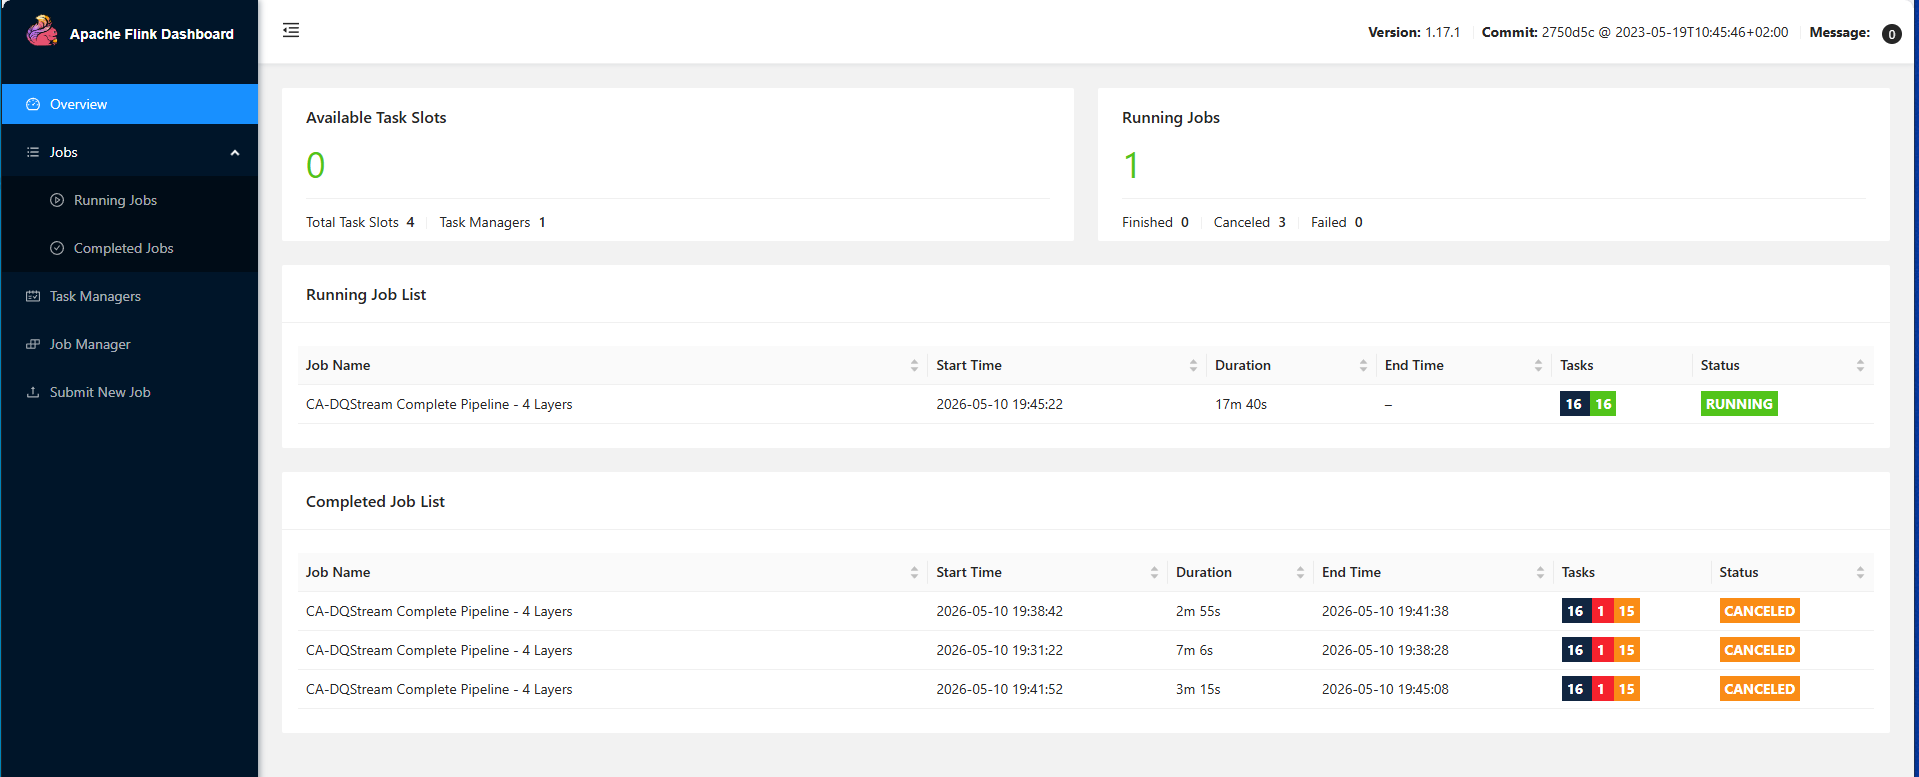
\includegraphics[width=0.85\textwidth]{figs/Thesis_Figures/flink2.PNG}}
\caption{Apache Flink cluster overview in the Web UI. The JobManager and TaskManagers form the distributed processing cluster, with processing slots allocated across worker nodes for parallel processing.}
\label{fig:flink_cluster_async}
\end{figure}

\textbf{Asynchronous Model Loading:} (1) Current model continues processing events during download/deserialization. (2) New model deserialized in a separate thread pool. (3) Atomic swap: once new model is ready, a volatile reference is atomically updated. (4) Processing thread reads from the volatile reference -- zero lock contention. (5) Old model dereferenced and garbage collected in background. This ensures zero-pipeline-interruption by maintaining two model versions during the transition period. The swap latency is sub-millisecond (atomic reference update).

\textbf{PyFlink Vectorized UDF as Micro-batching Optimization:} The ML scoring layer uses a mini-batching strategy (batch\_size=500) for: (1) \textbf{Python JVM Interoperability}: PyFlink requires serialization of each record across process boundaries (JVM $\leftrightarrow$ Python). Batch serialization amortizes IPC overhead across 500 records. (2) \textbf{Vectorized NumPy Operations}: Batch processing enables NumPy's BLAS-accelerated matrix operations, 10--100$\times$ faster than row-by-row Python loops. (3) \textbf{Throughput vs. Latency Trade-off}: CA-DQStream prioritizes throughput (15K-18K events/sec) over per-record sub-millisecond latency. This is explicitly a micro-batching design. For sub-10ms per-event requirements, alternative approaches (pure JVM-based ML, stateless scoring) should be considered.

\end{itemize}

Flink operators implement the pipeline stages:

\begin{longtable}{|m{4cm}|m{3.5cm}|m{5.5cm}|}
\hline
\textbf{Operator} & \textbf{Type} & \textbf{Function} \\ \hline
SchemaOperator & Stateless & NULL checks, range validation \\ \hline
BusinessRulesOperator & Stateless & 6 deterministic rules (Canary branch) \\ \hline
FeatureVectorizerOperator & Stateless & 15D context-aware features \\ \hline
MemStreamOperator & Stateful & Online AE + Memory scoring (Complex branch) \\ \hline
MetaAggregatorOperator & Stateful & 1-min aggregation by neighborhood \\ \hline
IECOperator & Stateful & ADWIN-U drift detection \\ \hline
\caption{Flink operators implementing the CA-DQStream pipeline.}
\label{tab:flink_operators}
\end{longtable}

\subsection{Apache Kafka Topics}

The pipeline uses 7 Kafka topics with 12 partitions each:

\begin{longtable}{|m{4cm}|m{9cm}|}
\hline
\textbf{Topic} & \textbf{Purpose} \\ \hline
taxi-nyc-raw & Raw NYC TLC records ingested from Parquet files \\ \hline
dq-schema-violations & Schema validation rejects (NULL, duplicates) \\ \hline
dq-hard-rule-violations & Business Rules violations (Canary branch) \\ \hline
dq-if-anomalies & Online Autoencoder + Memory Module detections (Complex branch) \\ \hline
dq-anomaly-scores & Raw anomaly scores for all records \\ \hline
dq-meta-stream & 6 aggregated quality metrics for IEC monitoring \\ \hline
if-model-updates & Serialized model bytes for Broadcast State updates \\ \hline
\caption{Apache Kafka topics in the CA-DQStream pipeline.}
\label{tab:kafka_topics}
\end{longtable}

\subsection{MinIO Data Storage}

All pipeline outputs are persisted to MinIO via Flink StreamingFileSink in Parquet format:

\begin{longtable}{|m{4cm}|m{9.5cm}|}
\hline
\textbf{Bucket} & \textbf{Description} \\ \hline
cadqstream-raw & Clean records with AE scores and context features \\ \hline
cadqstream-violations & Schema and Business Rules rejects \\ \hline
cadqstream-anomalies & Online AE + Memory Module detections with priority \\ \hline
cadqstream-metrics & DQ metrics per 1-minute window with IEC drift flags \\ \hline
cadqstream-drift & Drift events and IEC decisions \\ \hline
cadqstream-checkpoints & Flink checkpoints + ML model artifacts \\ \hline
mlflow-artifacts & MLflow tracking server artifacts \\
\hline
\caption{MinIO storage buckets for CA-DQStream.}
\label{tab:minio_schema}
\end{longtable}

Parquet format for columnar compression, bucket versioning enabled, automatic cleanup of raw data after 7 days. Flink incremental checkpoints (45-second intervals) and savepoints are stored via MinIO, with model artifacts versioned for rollback. MinIO provides S3 API compatibility, enabling migration to cloud S3 with minimal configuration changes.

\subsection{Prometheus \& Grafana Monitoring}

Prometheus scrapes metrics from Flink TaskManagers, MinIO, and Kafka. Key metrics: \texttt{if\_model\_version} tracks deployed model version; IEC-specific metrics include \texttt{iec\_drift\_events\_total}, \texttt{iec\_self\_adaptation\_tier}, and \texttt{if\_model\_broadcast\_updates\_total}.

Four Grafana dashboards provide operational visibility: DQ Overview (violation rates, NULL trends, IEC alerts), Online AE + Memory Module (anomaly counts, reconstruction distributions, $\Delta$\_Score), Business Rules (violations per type), and System Performance (throughput, Kafka lag, processing latency P50/P95/P99).

\subsection{Control Plane (FastAPI \& MLflow)}

The \textbf{Control Plane} manages model lifecycle and IEC action execution, decoupled from the real-time Flink streaming pipeline:

\textbf{MLflow (Experiment Tracking):} MLflow is used for tracking the initial warmup phase experiments (hyperparameters, training curves, validation metrics). The Online AE + Memory model lifecycle is simpler than IsolationForest: warmup phase $\rightarrow$ IEC-triggered memory update on drift detection. No periodic retraining job is needed during operation -- MLflow is used primarily for the warmup phase rather than ongoing model registry.

\textbf{FastAPI ML Service:} The FastAPI microservice exposes a lightweight REST endpoint (\texttt{/predict}, \texttt{/retrain}) that the IEC calls to trigger memory reset or AE warmup and receive updated model parameters. This decouples IEC decision-making (real-time, in Flink) from model adaptation (memory reset), maintaining sub-second stream processing latency while adaptation workflows run asynchronously in the background. The Action Replay Worker (Section 5.4.2) consumes IEC drift events from the \texttt{if-model-updates} Kafka topic and orchestrates the memory update pipeline without blocking the Flink stream.

\begin{itemize}
    \item \textbf{MLflow:} \texttt{http://localhost:5000} --- Experiment tracking, model versioning, registry lifecycle.
    \item \textbf{FastAPI:} \texttt{http://localhost:8000} --- IEC retrain endpoint, model parameter serving.
\end{itemize}

% ================================================
% 5.4 Optimization Techniques
% ================================================
\section{Optimization Techniques}

The ML scoring layer uses PyFlink Vectorized UDFs with mini-batching to break the Python GIL bottleneck. Scalar Python UDFs process one record at a time, serialized through the GIL, yielding only 240 events/sec on 12 parallel slots. Vectorized UDFs accumulate $B = 500$ records into a Pandas DataFrame, enabling NumPy to release the GIL during vectorized matrix operations. This achieves 3,920 events/sec (16$\times$ improvement), shifting the bottleneck from GIL contention to CPU-bound NumPy operations.

PyFlink IPC overhead (gRPC JVM $\leftrightarrow$ Python) costs 300$\mu$s per record. Mini-batching amortizes this: batch size $B = 200$ reduces per-record IPC from 300$\mu$s to 41.5$\mu$s (7.2$\times$ reduction). Combined with NumPy vectorization, the pipeline sustains 10,000--20,000 events/sec throughput.

Asynchronous model loading ensures zero-pipeline interruption: the current model continues processing while the new model downloads in a background thread, then atomically swaps via a volatile reference (sub-millisecond swap latency).

\textbf{LRU Cache:} FastAPI service caches loaded models (maxsize=10) to reduce model loading from 2--5s (cold) to $<$50ms (cache hit).

\textbf{State Size:} Deduplication operator stores Boolean flags per trip\_id within 7-day TTL, approximately 56 MB per slot with RocksDB overhead. Bloom filters reduce RocksDB I/O by 90\%.

\textbf{Action Replay Worker:} Failed IEC model update actions are retried with exponential backoff ($2^n$ seconds, up to 10 retries), then moved to Dead Letter Queue. An Update Lock (15-minute cooldown) prevents retry storms during sustained MLflow outages.


% ================================================
% 5.5 MLOps Integration
% ================================================
\section{MLOps Integration}

\subsection{MLflow Experiment Tracking}

CA-DQStream uses MLflow \citep{mlflow2024} for tracking the initial warmup phase experiments. The Online Autoencoder + Memory Module warmup phase is logged with:

\begin{itemize}
    \item \textbf{Parameters:} architecture (25D-50D-25D), activation, noise\_std, batch\_size, learning\_rate, epochs
    \item \textbf{Metrics:} training\_loss, validation\_loss, beta (95th percentile threshold), memory\_size
    \item \textbf{Artifacts:} AE weights (PyTorch state dict), memory vectors, scaler parameters
    \item \textbf{Tags:} warmup\_date, dataset\_version, clean\_data\_rate
\end{itemize}

MLflow tracking enables comparison of different AE architectures and hyperparameters during the warmup phase.

\subsection{Memory State Management}

The Online AE + Memory model uses a simpler lifecycle than IsolationForest:

\begin{itemize}
    \item \textbf{Warmup:} One-time initialization from ultra-clean data (AE weights + initial memory)
    \item \textbf{Online Learning:} Memory updates via FIFO replacement during normal operation
    \item \textbf{Drift Response:} Memory reset or AE warmup on fresh clean data (not full retraining)
\end{itemize}

The memory state is stored in Broadcast State and persists across Flink checkpoints. Unlike IsolationForest, no MLflow Model Registry is needed for ongoing updates -- the model adapts on-demand when drift is detected by IEC.

\subsection{CI/CD Pipeline}

CA-DQStream uses Docker Compose for containerized deployment with automatic versioning:

\begin{itemize}
    \item \textbf{Git tagging:} Each spec version (V1.9, V2.0) gets a git tag
    \item \textbf{Docker build:} Automated build of Flink job JAR and Python dependencies
    \item \textbf{Rolling deployment:} Flink savepoints enable pipeline upgrades without service interruption
\end{itemize}

% ================================================
% 5.6 Chapter Summary
% ================================================
\section{Chapter Summary}

This chapter detailed the engineering implementation of CA-DQStream's four core innovations (Chapter 3) on a distributed stack of Apache Flink, Kafka, MinIO, and Grafana.

\textbf{Key Implementation Highlights:}

\begin{itemize}
    \item \textbf{Four-Layer Processing Pipeline:} Schema Filter, Rendezvous (Canary + Complex), MetaAggregator, IEC
    \item \textbf{Infrastructure:} 7 Kafka topics, Flink (12 TaskManager slots), MinIO (7 buckets with Parquet output), Prometheus + Grafana (4 dashboards)
    \item \textbf{Optimization Techniques:}
        \begin{itemize}
            \item PyFlink Vectorized UDFs: 16$\times$ throughput improvement
            \item StreamingFileSink Parquet: efficient columnar storage on MinIO
            \item Broadcast State: atomic model swap without pipeline interruption
            \item MurmurHash3: 10--20$\times$ faster than MD5
            \item AggregateFunction pattern: prevents OOM on large windows
        \end{itemize}
    \item \textbf{MLOps Integration:} MLflow warmup tracking, Broadcast State model distribution, CI/CD with Docker Compose
\end{itemize}

The next chapter (Chapter 6) presents experimental validation of the four core innovations through 13 experiments spanning 72M records across 26 months.
